To apply these methods, a novel dataset was created, containing speech recordings of two speakers. 
All data were downloaded from YouTube using the open-source tool youtube-dl.
The first speaker is Grant Sanderson, a well-known educator and popularizer of mathematics. His dialect is 
standard American English.
The second is Rajamunickam Antonimuthu, a YouTuber operating a popular channel about science 
and technology news. His native language is Tamil, and is has a srong influence on his speech.
The speech samples of each speaker are relatively clean spontaneous speech. Depending on the exact 
process each uses for video creation, it may be at least partially scripted, but the nature of the speech 
samples is closest to spontaneous speech, especially compared to professional-quality read speech such as 
the LJSpeech corpus. In particular, there are more pauses and filler words.

For recognition and especially for synthesis, it is crucial to divide the longer speech files into smaller 
segments. To do this for the Antonimuthu corpus, subtitles were also scraped from the videos.
Because the subtitles are time-aligned to the video, and hence to the audio files, it was possible to 
divide on subtitle time stamps, combining segments up to a maximum length of 10 seconds.

For the Sanderson corpus, no subtitles were available, and so it was necessary to cut on silence. 
To accomplish this, the Python library \texttt{pydub} was used, with a silence threshold of -30 and 
a minimum silence length of 300 miliseconds. These values were found empirically to work best. 
As in the Atonimuthu corpus, smaller segments were combined as long as their combined length was 
less than 10 seconds.

The final corpus sizes were 10500 utterances for Sanderson and 2100 utterances for Antonimuthu, with average 
utterance length 4.49 and 6.34 seconds, respectively.

\subsection{Mel Spectrograms}
The mel spectrograms were generated in PyTorch as in the original Tacotron2 and Waveglow 
open-source implementations by NVIDIA [XX]. The hyperparameters were as follows:
\begin{itemize}
 \item input sampling rate: 22050 Hz
 \item number of mels: 80
 \item window length: 1024 (samples) $\approx$ 46.44ms
 \item filter length: 1024 (samples) $\approx$ 46.44ms
 \item shift (hop length): 160 (samples) $\approx$ 7.26ms
 \item minimum mel frequency: 0 Hz 
 \item maximum mel frequency: 8000 Hz
 \item audio bit depth: 32768 (15-bit)
\end{itemize}

\subsection{Phonetic Posteriorgrams}
Using the acoustic model described earlier and introduced in [XX], phonetic posteriorgrams were generated 
for each utterance, using the following hyperparameters:
\begin{itemize}
  \item input parameters:
    \begin{itemize}
      \item number of mels (for input): 80
      \item sampling rate: 22050 Hz
      \item window length: 64ms
      \item filter length: 64ms
      \item shift (hop length): 10ms
    \end{itemize}
  \item number of senones: 5816
  \item number of output phonemes: 40
  \item phoneme set: TIMIT reduced (40-phoneme) set
\end{itemize}

Examples:
\begin{itemize}
\item An Antonimuthu PPG representing the utterance \textit{``To overcome the drawbacks of SLM, 
Lawrence Livermore National University researchers''}:\\
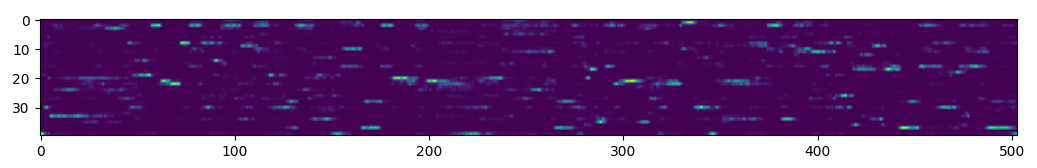
\includegraphics[width=\textwidth]{img/ppg_ant.png}
\item A Sanderson PPG representing the utterance \textit{``Geometric algebra, that is a whole other topic, uh, 
potentially for another day, but that's a - that's a really valid qustion''}:\\
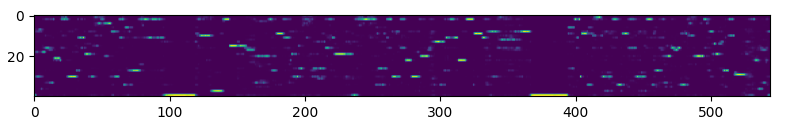
\includegraphics[width=\textwidth]{img/ppg_san.png}
\end{itemize}